\documentclass[a4paper,12p]{scrreprt}
\usepackage[left= 2.5cm,right = 2cm, bottom = 4 cm]{geometry}

% Standard Packages
\usepackage[utf8]{inputenc}
\usepackage[ngerman]{babel}
\usepackage[T1]{fontenc}
\usepackage{graphicx, subfig}
\usepackage{subcaption}
\usepackage{fancyhdr}
\usepackage[backend=biber]{biblatex}
\usepackage{listings}
\usepackage{xcolor}
\usepackage{float}
\addbibresource{references.bib}
\usepackage{enumitem}
\usepackage{mathptmx}
%\usepackage{lmodern}
%\usepackage{color}


%Für Usepackage Lisiting -> ermöglicht Code einzufügen:
\lstset{ 
  language=[Sharp]C,
  basicstyle=\small\ttfamily, % Kleine Schriftgröße für den Code
  keywordstyle=\color{blue},
  commentstyle=\color{green!40!black}, % Dunklere Grüntöne für Kommentare
  stringstyle=\color{orange},
  numbers=left,
  numberstyle=\tiny,
  numbersep=5pt,
  breaklines=true,
  showspaces=false,
  showstringspaces=false,
  frame=none,
  rulecolor=\color{black},
  captionpos=b
}



% zusätzliche Schriftzeichen der American Mathematical Society
\usepackage{amsfonts}
\usepackage{amsmath}
\usepackage[colorlinks=true, linkcolor=blue, citecolor=blue, urlcolor=blue]{hyperref}
% Für Abkürzungsverzeichniss
\usepackage[]{acronym}

% Begin des Dokumenntes
\begin{document}

\renewcommand{\thechapter}{\roman{chapter}}

\begin{figure}[h]
    \centering
    
\includegraphics[width = 0.55\textwidth]{img/Image_OTH.jpg}
    \label{fig: OTH Image}
\end{figure}


\begin{center}
    {\Huge {Vertiefung Microcomputertechnik} }
\end{center}

\vspace{2cm}

\noindent\makebox[\linewidth]{\rule{\linewidth}{0.4pt}}
\begin{center}
    {\Huge\textbf{CAN-TO-GO-SYSTEM} }
\end{center}
\noindent\makebox[\linewidth]{\rule{\linewidth}{0.4pt}}

\vspace{2cm}

\begin{center}
    {\Large {Von Michael Graml und Leonard Kreil} }
\end{center}

\vspace{1cm}

\begin{center}
    {\Large {Betruer/Prüfer: Prof. Dr. Stefan Krämer\\

             }}
\end{center}

\vspace{5cm}

\begin{center}
    {\Large Abgabe: 12.02.2024}
\end{center}

\newpage
\pagenumbering{Roman}
%Ab jetzt mit Kopf und Fußzeile
% ============= Kopf- und Fußzeile =============
\pagestyle{fancy}

%
\lhead{}
\chead{}
\rhead{\slshape \leftmark}
%%
\lfoot{VMC}
\cfoot{Michael Graml und Leonard Kreil}
\rfoot{\thepage}
%%
\renewcommand{\headrulewidth}{0.4pt}
\renewcommand{\footrulewidth}{0.4pt}

%\include{02_Sperrvermerk_Erklärung}
%\include{03_Zusammenfassung}
\addsec{Zusammenfassung / Abstract}
\label{sec:zusammenfassung}
Das ist meine Zusammenfassung

\minisec{Abstract}
\label{abstract}

lalalal

%Inhaltsverzeichnis
\include{10_Abkürzungsverzeichniss}
\tableofcontents
\thispagestyle{fancy}
\pagenumbering{arabic} % Wechsel zu arabischen Seitenzahlen
\renewcommand{\thechapter}{\arabic{chapter}} % Ändert die Kapitelnummerierung auf römische Ziffern



%\include{07_CPCOM}
\chapter{Einleitung}
\label{sec:Einleitung}
\noindent Die Arbeit wurde gemeinschaftlich von Michael Graml und Leonard Kreil durchgeführt. Sollten Unterschiede in der Bearbeitung einzelner Abschnitte vorliegen, sind diese in den jeweiligen Kapiteln gekennzeichnet.\\

\begin {centering}
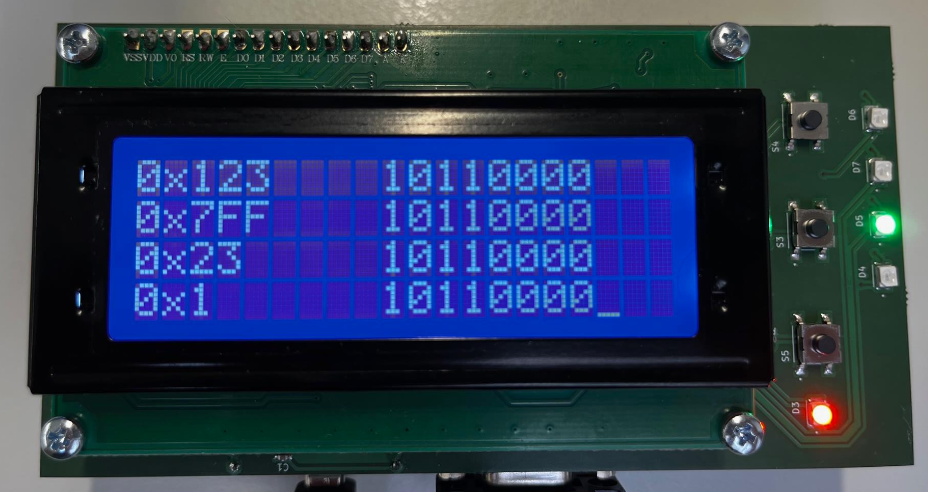
\includegraphics[width=0.75\textwidth]{img/Can_to_go_system.png}
\captionof{figure}{CAN-TO-GO System}
\label{fig: CAN-to-go System}
\end {centering}  


\section{CAN}
Controller Area Network (CAN) ist ein standardisiertes, robustes Fahrzeugbussystem, das für die Kommunikation zwischen verschiedenen Steuergeräten (ECUs) in Fahrzeugen und anderen industriellen Anwendungen konzipiert wurde. Es ermöglicht den zuverlässigen Datenaustausch mit hoher Fehlertoleranz und geringer Latenz, was besonders in Echtzeitanwendungen wichtig ist. CAN-Busse verwenden ein Nachrichtenbasiertes Protokoll, bei dem jede Nachricht eine eindeutige ID hat, die ihre Priorität bestimmt. Dieses System ist besonders nützlich bei der Diagnose von Netzwerkproblemen, da die Priorisierung von Nachrichten und Fehlererkennungsmechanismen die Fehlersuche erleichtern. Die physikalischen Aspekte des CAN-Busses, wie Abschlusswiderstände und die Verkabelung (CANL/CANH), sind ebenfalls entscheidend für die Netzwerkintegrität. Die Anpassungsfähigkeit hinsichtlich der Baudrate und die Unterstützung verschiedener Netzwerkstrukturen machen CAN vielseitig einsetzbar.\\

\section{Can-Datentelegram}
\begin{figure}[h]
    \centering
    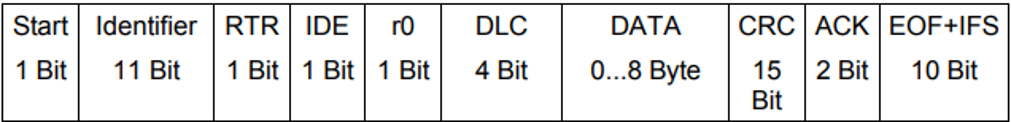
\includegraphics[width = 0.55\textwidth]{img/standard_datenframe.png}
    \caption{Standard Datentelegram \cite{3}}
    \label{fig: Standard Datentelegram}
\end{figure}
\begin{figure}[h]
    \centering
    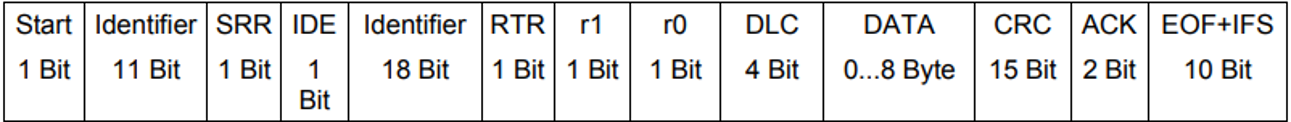
\includegraphics[width = 0.55\textwidth]{img/extended_datenframe.png}
    \caption{Extended Datentelegram \cite{3}}
    \label{fig: Extended Datentelegram}
\end{figure}

\noindent Ein CAN-Datentelegramm beginnt mit einem Startbit zur Synchronisation der kommunizierenden Geräte. Der Identifier gibt die Nachrichtenpriorität an und dient der Busarbitrierung, wobei das RTR-Bit zwischen einem Daten- und einem Datenanforderungstelegramm unterscheidet. IDE ist die Identifier Extension, die anzeigt, ob ein Standard- (11-Bit-Identifier siehe Abbildung \ref{fig: Standard Datentelegram}) oder ein Extended-Frame (29-Bit-Identifier siehe Abbildung \ref{fig: Extended Datentelegram}) verwendet wird. DATA enthält die eigentlichen Nutzdaten. CRC ist eine Prüfsumme zur Fehlererkennung. ACK signalisiert den korrekten Empfang der Nachricht. EOF und IFS kennzeichnen das Ende des Datentelegramms und den erforderlichen Abstand bis zum nächsten Frame. Im Extended Frame ersetzt das SRR-Bit das RTR-Bit des Standard Frames, und die DLC-Information gibt die Länge der Daten an.\\

\section{Anfordderungsanalyse}
\noindent Das "Can to Go"-System wird entwickelt, um Anwendern bei Problemen beim Aufbau eines CAN-Busses zu assistieren und zu diagnostizieren, wo genau die Schwierigkeiten liegen. Es dient als funktionssicherer CAN-Teilnehmer, der in der Lage ist, CAN-Nachrichten zuverlässig zu lesen und zu interpretieren. Kernmerkmale umfassen ein Anschlusskästchen mit SUB-D-Stecker und Status-LEDs, die den Betriebszustand des CAN-Busses anzeigen. Ein optionaler Abschlusswiderstand, der nach Bedarf zugeschaltet werden kann, sowie die Anpassungsfähigkeit der Baudrate gehören ebenfalls zu den wesentlichen Anforderungen. Darüber hinaus wird das System die CAN-Nachrichten und die zugehörigen Sender-IDs sichtbar machen.\\


\section{Endprodukt}

\subsection{Überblick}
\noindent Das Endprodukt des "Can to Go"-Systems bildet eine fortschrittliche Lösung für die Überwachung und Diagnose von CAN-Bussystemen. Es integriert die erforderlichen Funktionen aus der Anforderungsanalyse mit zusätzlichen Merkmalen, die seine Benutzerfreundlichkeit und Vielseitigkeit erhöhen.\\

\subsection{Hauptmerkmale}
\begin{itemize}
    \item \textbf{Anschluss und Konnektivität:} Ausgestattet mit einem Anschlusskästchen und SUB-D-Stecker, verfügt das System über Status-LEDs, die den Betriebszustand des CAN-Busses anzeigen. Diese visuellen Indikatoren erleichtern das schnelle Erkennen von Verbindungsproblemen.
    
    \item \textbf{Funktionalität und Anpassungsfähigkeit:} Ein optionaler Abschlusswiderstand kann nach Bedarf hinzugeschaltet werden. Die Anpassbarkeit der Baudrate gewährleistet eine breite Kompatibilität mit verschiedenen CAN-Bus-Konfigurationen.
    
    \item \textbf{Display und Anzeige:} Das Gerät umfasst ein kleines Display, das CAN-Nachrichten anzeigt. Dieses Display bietet eine direkte, wenn auch begrenzte, Einsicht in die CAN-Kommunikation.
    
    \item \textbf{Energieversorgung:} Es enthält keinen eigenen Akku, kann aber durch eine externe Powerbank mit Energie versorgt werden, was eine flexible Nutzung ermöglicht.
\end{itemize}   

\subsection{Zusätzliche Funktionen}
\begin{itemize}
 \item \textbf{App- und Web-Integration:} Ergänzend zum kleinen Display des Geräts ermöglichen eine App und eine Website die detaillierte Ansicht von CAN-Nachrichten, inklusive Zeitstempeln. Diese digitalen Plattformen erlauben eine umfassende Analyse da sie eine größere Benutzeroberfläche als das Display bieten.
\end{itemize}   



\chapter{Hardwareaufbau und Leiterplattenentwurf}
\label{sec:Hardware}



\noindent Der Hardwareaufbau dieses Projekts basiert auf einer sorgfältig gestalteten Leiterplatte, die alle erforderlichen Hardwarekomponenten integriert. Der Prozess des Leiterplattenentwurfs wurde mittels KiCad, einem Open-Source-Tool für PCB-Design, durchgeführt.\\

\begin {centering}
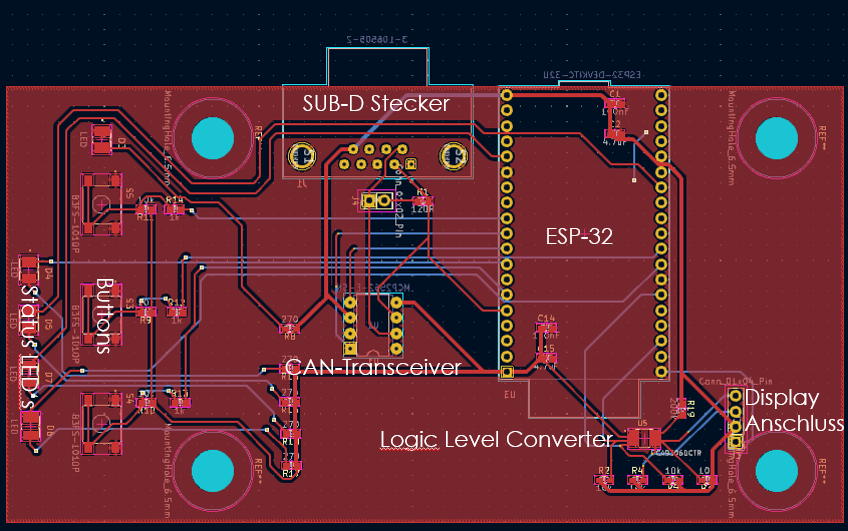
\includegraphics[width=0.75\textwidth]{img/Leiterplate.png}
\captionof{figure}{Leiterplattenentwurf}
\label{fig: Leiterplattenentwurf}
\end {centering}  

\section{Leiterplattenentwurf}
\subsection{Entwurfsprozess}
\begin{itemize}
    \item \textbf{Komponentenauswahl und -platzierung:} Zunächst wurden die benötigten elektronischen Bauteile ausgewählt und in den Schaltplan von KiCad integriert. Jedem Bauteil wurde ein entsprechender Footprint zugewiesen. Diese Footprints sind entscheidend, da sie die physische Größe und Platzierung der Komponenten auf der Leiterplatte bestimmen.
    \item \textbf{Layoutgestaltung:} Im Anschluss wurden die Bauteile sorgfältig auf der Leiterplatte platziert. Besonderes Augenmerk lag dabei auf der logischen Gruppierung der Komponenten und der Minimierung der Leitungslängen, um Effizienz und Signalintegrität zu gewährleisten.
\end{itemize}

\subsection{Herstellung und Bestückung}
\begin{itemize}
    \item \textbf{Leiterplattenbestellung:} Die Leiterplatte wurde bei Aisler in Auftrag gegeben. Die Entscheidung, die Bauteile separat zu bestellen, wurde aus Kostengründen getroffen.
    \item \textbf{Komponentenbeschaffung:} Die einzelnen elektronischen Bauteile wurden von Mouser Electronics bezogen.
    \item \textbf{Bestückung der Leiterplatte:} Die Montage der Bauteile auf der Leiterplatte erfolgte mittels Lötpaste. Bei diesem Prozess wurde besonders auf Präzision und Sauberkeit geachtet, um Kurzschlüsse oder Fehlverbindungen zu vermeiden, die die Funktionalität der Schaltung beeinträchtigen könnten.
\end {itemize}

\noindent Die detaillierte Kostenaufstellung der einzelnen Bauteile sowie der Leiterplatte selbst ist in Tabelle \ref{tab:Stückliste} dargestellt. Diese Übersicht bietet eine klare Kostentransparenz und erleichtert die Nachvollziehbarkeit des Projekts.\\

\section{ESP32}
Der ESP32 ist das Herzstück unseres eingebetteten Systems und übernimmt die zentrale Verarbeitung und Koordination aller Aufgaben. Als hochintegrierter Mikrocontroller verbindet er verschiedene Elemente des Systems, wie die CAN-Schnittstelle, das Display, Status-LEDs und Taster, zu einem funktionierenden Ganzen.\\

\noindent Im Rahmen der CAN-Kommunikation liest der ESP32 die über den CAN-Bus gesendeten Nachrichten und verarbeitet diese. Außerdem steuert ESP32 das Display über das I2C-Protokoll, wobei ein Logikpegelwandler für die Anpassung der unterschiedlichen Spannungsniveaus zwischen dem 3,3-Volt-System des ESP32 und dem 5-Volt-Display verwendet wird.\\

\noindent Die Taster sind über Pull-up-Widerstände an den ESP32 angeschlossen und ermöglichen es den Benutzern, durch einfaches Drücken die Konfigurationseinstellungen vorzunehmen. Der ESP32 interpretiert diese Eingaben und führt die entsprechenden Aktionen aus, wie beispielsweise das Wechseln der Baudrate.\\

\noindent Durch seine Vielseitigkeit und leistungsstarke Verarbeitungskapazität bildet der ESP32 das Rückgrat des Systems.\\

\begin {centering}
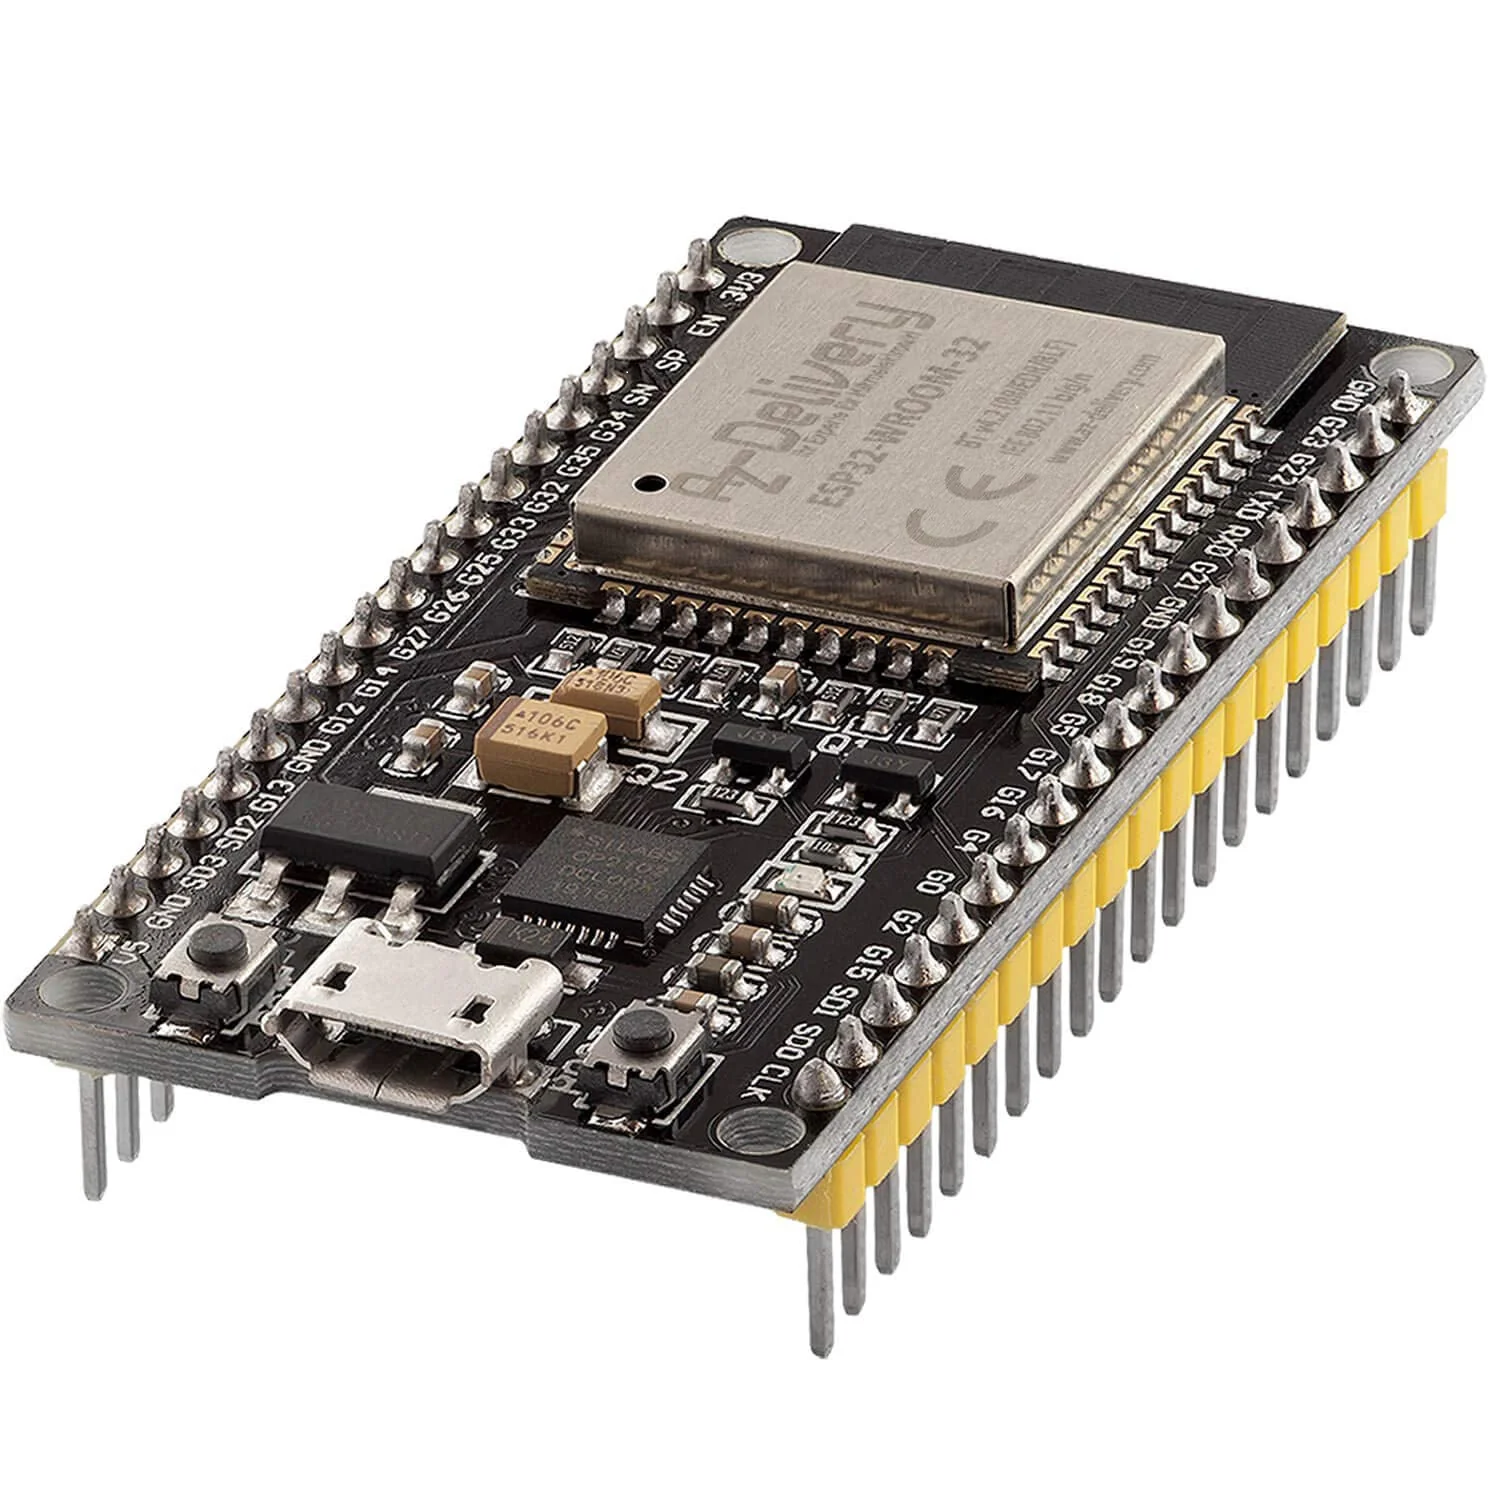
\includegraphics[width=0.5\textwidth]{img/ESP32.png}
\captionof{figure}{ESP32 \cite{1}}
\label{fig: ESP32}
\end {centering}  

\section{Display}
\noindent Das Display dient in unserem eingebetteten System als primäre Benutzerschnittstelle, indem es die Baudrateneinstellungen im Konfigurationsmodus sowie die CAN-Nachrichten und ihre Identifier im Operationsmodus anschaulich visualisiert. In unserem System erfolgt die Kommunikation zwischen dem ESP32-Mikrocontroller und dem Display über das I2C-Protokoll (Inter-Integrated Circuit), einem weit verbreiteten Kommunikationsstandard, der für seine Einfachheit und Effizienz in der synchronen seriellen Datenübertragung bekannt ist.\\

\noindent I2C nutzt nur zwei Leitungen – eine für das serielle Daten-Signal (SDA) und eine für das serielle Clock-Signal (SCL) – und ermöglicht es dem Mikrocontroller, mehrere Geräte über einen einzigen Bus zu steuern, wobei jedes Gerät über eine einzigartige Adresse identifiziert wird. Dieser Bus ermöglicht eine bidirektionale Kommunikation, was bedeutet, dass der ESP32 Daten an das Display senden und gleichzeitig Statusinformationen vom Display empfangen kann. \\

\noindent Da der ESP32 mit einer Logikspannung von 3,3 Volt arbeitet, während das Display für eine Betriebsspannung von 5 Volt ausgelegt ist, wurde ein Logikpegelwandler verwendet, um die Signale zwischen diesen beiden Spannungsebenen zu übersetzen (siehe Abschnitt ...). Zusätzlich wird für die physische Verbindung des Displays ein serieller I2C/TWI-Schnittstellenadapter verwendet, der bereits im Lieferumfang des Kits enthalten ist.\\

\begin{centering}
  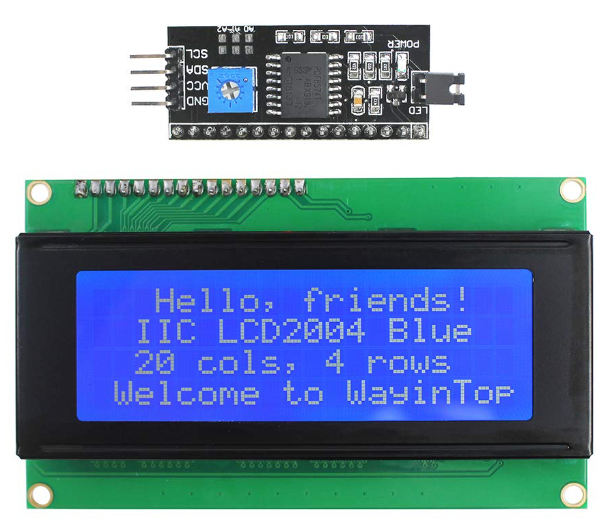
\includegraphics[width=0.5\textwidth]{img/Display.png}
  \captionof{figure}{Display mit Displayanschluss \cite{4}}
  \label{fig: Display}
\end{centering}

\section{SUB-D Stecker}
\noindent Der SUB-D-Stecker dient der Einbindung von CAN-Nachrichten in das betreffende System. Über diese Schnittstelle lässt sich das 'CAN to go'-System mit dem zu testenden CAN-Netzwerk verbinden. Die Konfiguration der Pin-Belegung ist spezifisch angeordnet: CAN-Low ist an Pin 2, CAN-High an Pin 6, der Masseanschluss (GND) an Pin 3 und die Versorgungsspannung von +5V an Pin 9 angebunden. Abhängig von den systemseitigen Erfordernissen kann ein 120-Ohm-Terminierungswiderstand zwischen CAN-Low und CAN-High integriert werden, um die Signalintegrität zu gewährleisten. Die Schaltung dieses Terminierungswiderstandes erfolgt über den Anschluss J4, der in der grafischen Darstellung blau umkreist ist (siehe Abbildung \ref{fig: SUB-D Stecker und Terminierungswiderstand}).\\

\begin{centering}
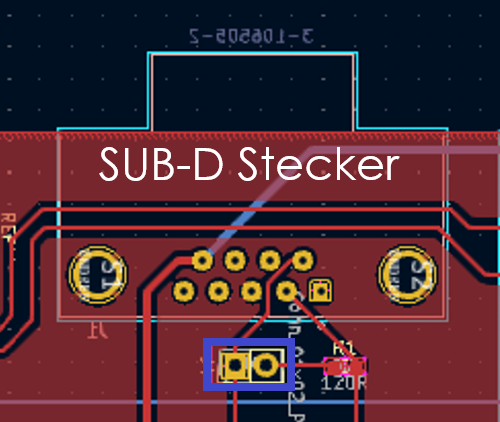
\includegraphics[width=0.5\textwidth]{img/SUB_D_zuschaltbarer_widerstand.png}
\captionof{figure}{SUB-D Stecker und Terminierungswiderstand}
\label{fig: SUB-D Stecker und Terminierungswiderstand}
\end{centering}

\section{Can Transciever}
\noindent Der MCP2562-E-P Transceiver spielt eine zentrale Rolle im Hardwareaufbau für die CAN-Kommunikation, indem er die Signale aus dem CAN-Netzwerk in digitale Signale umwandelt, die vom ESP32-Mikrocontroller verarbeitet werden können. Der Transceiver agiert als Bindeglied zwischen den differenziellen Signalen des CAN-Busses und den digitalen I/O-Pins des ESP32. Er wandelt die auf dem CAN-Bus empfangenen Hoch- und Niedrigzustände (CAN\_H und CAN\_L) in logische Pegel um, die der Mikrocontroller verstehen kann. Dies ermöglicht eine reibungslose und zuverlässige Kommunikation zwischen den CAN-Geräten und dem Mikrocontroller.\\

\noindent Zur Implementierung dieser Funktion müssen die CAN\_H und CAN\_L Leitungen des MCP2562-E-P an die entsprechenden Leitungen des CAN-Busses angeschlossen werden. Die Tx und Rx Pins des Transceivers werden dann mit den entsprechenden digitalen I/O-Pins des ESP32 verbunden, um die Kommunikation zu ermöglichen. Die genaue Pinbelegung und Konfiguration ist in dem Datenblatt des Transceivers zu finden \cite{2}.\\

\section{Status LEDS}
In unserem eingebetteten System fungieren Leuchtdioden (LEDs) als visuelle Indikatoren für verschiedene Zustände des Gerätes. Ihre Hauptfunktion besteht darin, den Benutzer über den aktuellen CAN Status zu informieren. Die LEDs sind über 270-Ohm-Widerstände an den Mikrocontroller angeschlossen, um den Strom zu begrenzen, der durch die LEDs fließt. Dies schützt die LEDs vor Überstrom, der sie beschädigen könnte, und stellt sicher, dass sie innerhalb ihrer spezifizierten Stromgrenzen betrieben werden, was zu einer längeren Lebensdauer und zuverlässigeren Leistung führt.\\

\begin{itemize}
  \item \textbf{Orange LED (D3):} Die Beleuchtung dieser LED zeigt an, dass das System mit Strom versorgt wird, und dient somit als Power-On-Statusanzeige.
  \item \textbf{Rote   LED (D4):} Diese LED beginnt zu leuchten, wenn die Nachrichten auf dem angeschlossenen CAN-Bus nicht interpretiert werden können. Dies dient als Indikator für Störungen oder Fehler im CAN-System.
  \item \textbf{Grüne  LED (D5):} Die grüne LED signalisiert, dass die Nachrichten des CAN-Bus korrekt interpretiert werden und das System ordnungsgemäß funktioniert.
  \item \textbf{Blaue  LED (D6):} Diese LED beginnt zu blinken wenn eine CAN Nachricht gesendet wird.
  \item \textbf{Blaue  LED (D7):} Diese LED beginnt zu blinken wenn eine CAN Nachricht empfangen wird.
\end{itemize}

\noindent Die Ansteuerung der LEDs erfolgt direkt durch den ESP32-Mikrocontroller, der die Fähigkeit besitzt, seine GPIO-Pins (General Purpose Input/Output) als Ausgänge zu konfigurieren. Durch Programmierung des Mikrocontrollers kann jeder dieser Pins einen High- oder Low-Zustand annehmen, wobei High bedeutet, dass der Pin eine Spannung ausgibt, die ausreicht, um die LED zum Leuchten zu bringen. Der Low-Zustand hingegen unterbricht den Stromfluss, sodass die LED erlischt.\\


\section{Buttons}
\noindent In unserem System werden Taster (Buttons) als Eingabemittel für Benutzerinteraktionen verwendet. Sie ermöglichen es dem Benutzer, Steuersignale an den Mikrocontroller zu senden, der diese dann entsprechend der programmierten Logik interpretiert. Die Taster sind einfache, aber effektive Komponenten in der Mensch-Maschine-Interaktion innerhalb eingebetteter Systeme.\\

\noindent Die drei Taster sind jeweils über einen Pull-up-Widerstand an eine Versorgungsspannung (+3V3) angeschlossen. Dies sorgt dafür, dass das Signal am entsprechenden Eingangspin des ESP32 standardmäßig auf einem hohen Logikniveau (High) liegt. Wird der Taster gedrückt, schließt sich der Stromkreis, und der Eingangspin wird auf das niedrige Logikniveau (Ground) gezogen.Die zusätzlichen Widerstände (R12, R13, R14) dienen als Strombegrenzungswiderstände und schützen den Mikrocontroller vor hohen Strömen, die beim Schließen des Tasterkreises entstehen könnten. Diese Anordnung wird als Pull-up-Konfiguration bezeichnet und ist eine gängige Methode, um den Zustand eines Eingangspins zu definieren, wenn kein Signal anliegt.\\

\noindent Im Konfigurationsmodus unseres Systems ermöglichen es die Taster dem Benutzer, die Einstellungen für die Baudrate zu navigieren und zu bestätigen. Jeder Taster hat eine spezifische Rolle:

\begin{itemize}
  \item \textbf{Taster S3:} Dieser Taster ermöglicht es dem Benutzer, auf dem Display nach oben zu navigieren.
  
  \item \textbf{Taster S4:} Der Taster S4 bietet dem Benutzer die Möglichkeit, Einstellungen zu bestätigen, wie beispielsweise die Auswahl der Baudrate.
  
  \item \textbf{Taster S5:} Sollte der Benutzer im Display nach unten navigieren müssen, wird Taster S5 verwendet.
\end{itemize}


\section{Logic Level Converter}
\noindent Im Kontext eingebetteter Systeme spielt die Signalintegrität zwischen verschiedenen elektronischen Komponenten eine entscheidende Rolle. Verschiedene Bauteile operieren oft mit unterschiedlichen Logikpegeln, was bedeutet, dass die Spannung, die ein High-Signal (logische "1") repräsentiert, zwischen diesen Komponenten variieren kann. Um eine korrekte und sichere Kommunikation zwischen solchen Bauteilen zu gewährleisten, werden Logikpegelwandler eingesetzt.\\

\noindent In unserem System haben wir den Logikpegelwandler PCA9306DCTR implementiert, um eine bidirektionale Schnittstelle zwischen dem 3,3-Volt-Logikpegel des ESP32-Mikrocontrollers und dem 5-Volt-System des Displays zu schaffen. Dieser Schritt ist notwendig, da eine direkte Verbindung ohne entsprechende Anpassung der Spannungsniveaus zu einem für das Display nicht detektierbaren Signal führen würde.\\

\noindent Der PCA9306DCTR zeichnet sich durch eine Schaltung aus, die mit Transistoren und Pull-up-Widerständen ausgestattet ist. Diese Komponenten sind präzise konfiguriert, um eine nahtlose Umwandlung von Signalen zu ermöglichen: Ein High-Signal wird von der niedrigeren Spannung des ESP32 (3,3 V) auf die höhere Spannung des Displays (5 V) angehoben und umgekehrt. Diese Funktionsweise stellt sicher, dass es zu keiner Signalverzerrung oder Beeinträchtigung der Signalintegrität kommt. Der PCA9306DCTR ermöglicht so eine reibungslose und sichere Interaktion zwischen dem ESP32 und dem Display, was für die Zuverlässigkeit und Robustheit des Gesamtsystems unerlässlich ist.\\

\section{Bypass Kondensatoren}
Die Stabilität und Zuverlässigkeit der Stromversorgung sind für die Funktionalität des Systems von entscheidender Bedeutung. Um dies zu gewährleisten, werden Bypass- oder Abblockkondensatoren an den Spannungsausgängen des ESP32 eingesetzt. Diese Kondensatoren spielen eine zentrale Rolle bei der Minimierung von Spannungsschwankungen und elektrischem Rauschen, die die Leistung und das Verhalten des Systems negativ beeinflussen können.\\

\noindent \textbf{Stabilisierung der Versorgungsspannung}\\
\noindent Bypass-Kondensatoren dienen als lokale Energiereserven, die direkt an den Spannungsausgängen des ESP32 positioniert sind. Sie bieten eine schnelle Reaktionsquelle für Energie, um die Versorgungsspannung konstant zu halten, wenn der Mikrocontroller zwischen energieintensiven Prozessen wechselt.\\

\noindent \textbf{Rauschunterdrückung}\\
\noindent Elektronische Schaltungen sind anfällig für Rauschen und transiente Störungen, die von anderen Teilen der Schaltung oder externen Quellen stammen können. Die Bypass-Kondensatoren filtern effektiv das hochfrequente Rauschen heraus, indem sie es zur Masse ableiten, und verhindern so, dass es die Leistung des Mikrocontrollers beeinträchtigt.\\

\noindent \textbf{Reaktion auf Lastwechsel}\\
\noindent Der ESP32 kann plötzliche Lastwechsel erfahren, beispielsweise beim Übergang von einem niedrigen Stromverbrauchszustand zu einer hohen Rechenleistung. Bypass-Kondensatoren helfen, solche Lastwechsel zu bewältigen, indem sie sofort Energie liefern oder aufnehmen, um die Versorgungsspannung zu stabilisieren.\\

\noindent \textbf{Dimensionierung der Bypass-Kondensatoren}\\
\noindent Zwei Arten von Bypass-Kondensatoren werden typischerweise verwendet:
\begin{itemize}
  \item \textbf{Kondensatoren mit 100nF:} Diese sind für die Filterung hochfrequenter Störungen ausgelegt und sind ein Standard in vielen Schaltkreisen, die integrierte Schaltungen enthalten.
  \item \textbf{Kondensatoren mit 4,7µF:} Sie bieten eine größere Kapazität für die Energieaufnahme und sind besonders effektiv, um die Spannung bei größeren Lastwechseln zu stabilisieren.
\end{itemize}

\noindent Diese Kondensatoren ergänzen sich gegenseitig, wobei der 100nF-Kondensator schnelle, kurzzeitige Schwankungen abfängt, während der 4,7µF-Kondensator für länger anhaltende Stabilität sorgt. Die Kombination beider Typen stellt sicher, dass der ESP32 unter allen Betriebsbedingungen effizient und fehlerfrei arbeiten kann.



\section{Stückliste}

\begin{table}[htbp]
  \begin{center} % Zentriert die Tabelle
      \begin{tabular}{cccc} % Definiert die Anzahl und Ausrichtung der Spalten (hier: zwei zentrierte Spalten)
          \hline % Horizontale Linie oberhalb der Tabelle
          Name & Bauteilbezeichnung & Spezifikationen & Menge \\ % Inhalt der Tabelle, & trennt die Spalten
          \hline % Horizontale Linie oberhalb der Tabelle
          ESP32 & ESP-32 Dev Kit C V4 &  & 1\\
          Widerstand  &  & 270 Ohm & 5 \\
          Widerstand &  & 120 Ohm & 1 \\
          Widerstand &  & 1k Ohm & 3 \\
          Widerstand &  & 10k Ohm & 7\\
          Widerstand &  & 200k Ohm & 1\\
          Kondensator &  & 4.7 µF & 2\\
          Kondensator &  & 100nF & 2\\
          LED &  & & 5\\
          SUB-D Stecker & 3-106505-2 & & 1\\
          Button & B3FS-1010P & & 3\\
          CAN Transceiver & MCP2562-E-P & & 1\\
          Logic Level Converter & PCA9306DCTR & & 1\\
          Display & WayinTop 20x4 2004 LCD & & 1\\
          Display Anschluss & TWI IIC I2C LCD & & 1\\
          Leiterplatte &  & & 1\\
          \hline % Horizontale Linie unterhalb der letzten Zeile
      \end{tabular}
  \caption{Stückliste der verwendeten Bauteile}
  \label{tab:Stückliste}
  \end{center}
  \end{table}

% Verzeichnis der Quellen
\printbibliography
% Verzeichnis der Bilder
\listoffigures
% Verzeichnis der Listings
\lstlistoflistings

\end{document}